
\section{Experimental evaluation}
\label{sec:experiments}

This section presents several experiments to evaluate the performance of \FAMA and the quality of the learned models. Whenever applicable, we will consider scenarios with both known and unknown plan horizon to draw conclusions at both levels of complexity.

After presenting the setup of the experiments in section \ref{setup}, we introduce three experiments that measure different aspects like the minimal number of traces necessary to obtain good quality models (section \ref{size_knowledge}), a comparison of the quality of models obtained by \FAMA compared to \ARMS (section \ref{compare_ARMS}) and an analysis of the quality of models when using a very small number of input traces in section \ref{minimal} In these three experiments, the quality of the models is measured using the syntactic-based precision and recall metrics presented in section \ref{syntactic_precision_recall}, that is, we measure the precision and recall of the learned models with respect to the GTM for each domain. Finally, the syntactic evaluation of section \ref{minimal} is compared against a semantic evaluation, i.e. how well the learned models are able to reproduce the input plan traces, in section \ref{semantic}.



\subsection{Setup}
\label{setup}

We evaluate \FAMA on 15 IPC domains that satisfy the \strips\ requirement~\cite{fox2003pddl2}, all taken from the {\sc planning.domains} repository~\cite{muise2016planning}. Table \ref{tab:domain_features} presents the features of the tested domains that affect the size of the planning task $P_\Lambda$ that results from the compilation. For each domain, the columns report, from left to right, the number of actions, the number of predicates, the maximum arity of the actions, and the maximum arity of the predicates.

The details of our experimental setup are the following:

\begin{itemize}
\item {\bf Plan traces}. For each domain, we generated 10 plan traces, each with 10 actions and 10 intermediate states, using random walks. Depending on the experiment, the traces are used for training or testing purposes (more details on this issue are provided at the particular experiment).

\item {\bf Planner}. The classical planner we used to solve the instances of $P_\Lambda$ that result from our compilations is {\sc Madagascar}~\cite{rintanen2014madagascar}. We used {\sc Madagascar} for several reasons:

  \begin{enumerate}
  \item Other planners such as {\sc FastDownward} were also tested but provided worse experimental results
  \item The ability of {\sc Madagascar} to deal with instances populated with dead-ends, such as our compiled problem $P_\Lambda$, is very helpful~\cite{lopez2015deterministic}.
  \item A SAT-based planner like {\sc Madagascar} is particularly suitable for tasks where the observed plan trace $\tau$ determines the horizon of the solution plan (case 1 presented in section \ref{task_definition}). In this case, a SAT-based planner solves the prefix of the solution plan in two time steps because the actions for inserting preconditions can be applied in parallel in a single time step and the same for the actions inserting the effects. 
  \end{enumerate}

\item {\bf Hardware}. All experiments were run on an Intel Core i5 3.50 GHz x 4 with 16 GB of RAM.

\item {\bf Reproducibility}. We make fully available the compilation source code, the evaluation scripts and the used benchmarks at this repository {\em https://github.com/daineto/meta-planning} so any experimental data reported in the paper is fully reproducible.
\end{itemize}

\begin{table}[hbt!]
	\begin{footnotesize}			
		\begin{center}
			\begin{tabular}{l|c|c|c|c|}	
				& \multicolumn{4}{c|}{Domain features}\\ \cline{2-5}
				& {\bf \# actions} & {\bf \# predicates} & {\bf max action arity} & {\bf max predicate arity}  \\
				\hline
				Blocks & 4 & 5 & 2 & 2  \\
				Driverlog & 6 & 5 & 4 & 2  \\
				Ferry & 3 & 5 & 2 & 2  \\
				Floortile & 7 & 10 & 4 & 2  \\
				Grid & 5 & 9 & 4 & 2  \\
				Gripper & 3 & 4 & 3 & 2  \\
				Hanoi & 1 & 3 & 3 & 2  \\
				Miconic & 4 & 6 & 2 & 2  \\
				Npuzzle & 1 & 3 & 3 & 2  \\
				Parking & 4 & 5 & 3 & 2  \\
				Rovers & 9 & 25 & 6 & 3 \\
				Satellite & 5 & 8 & 4 & 2  \\
				Transport & 3 & 5 & 5 & 2  \\
				Visitall & 1 & 3 & 2 & 2  \\
				Zenotravel & 5 & 4 & 5 & 2
			\end{tabular}
		\end{center}
	\end{footnotesize}			
	\caption{\small Feature description of the domains used in the experiments.}
	\label{tab:domain_features}	
\end{table}

\subsection{Impact of the size of the input knowledge}
\label{size_knowledge}

This experiment evaluates the impact of $\left|\mathcal{T}\right|$, the size of the input knowledge, on the performance of \FAMA in order to:

\begin{enumerate}
	\item Identify the minimal amount of input knowledge required by \FAMA to learn sound and complete models,
	\item Evaluate the scalability of \FAMA with respect to the size of the input knowledge.
\end{enumerate}

The experiment analyzes the evolution of the CPU-time and the precision and recall of the learned models wrt the GTM as $|\mathcal{T}|$ increases from 1 to 10 plan traces. To keep the experiment practicable, we introduced a 1000s timeout, after which the learning process is killed and a score of $0$ is given to both the precision and recall of the learned model. We defined two case studies:

\begin{itemize}
	\item \textbf{\FO action sequence and \PO state trajectory (known plan horizon)}: This is the common case addressed by most of the state-of-the-art learning approaches, which corresponds to a scenario where the plan horizon is given by the action sequence. In this experiment we assume a degree of observability of only 10\% for the state trajectory, meaning that each literal of a state has a 10\% chance of being observed.
	\item  \textbf{\NO action sequence and \NO state trajectory (unknown plan horizon)}: In this case study, both the input action sequence and state trajectory are {\em empty} and the length of the plan is unknown. Only the initial and final states are observed; i.e., $\tau = \tup{s_0, s_m}, \forall \tau \in \mathcal{T}$.
\end{itemize}

Figures \ref{fig:np_quality} and \ref{fig:np_time} show the quality of the models and computation time, respectively, for the case \FO/\PO. The values plotted in these figures are averages over the 15 domains. In Figure \ref{fig:np_quality} we see that, after three traces, precision stabilizes at 0.84 whereas recall stabilizes at 0.95. These results show that \FAMA does, in fact, not need big amounts of input knowledge to learn sound and complete models as opposite to other approaches in the literature where models are learned using around 100 traces (see Table \ref{table:models_comparison2}).

Figure \ref{fig:np_time} displays the scalability of \FAMA. Interestingly, we can observe an exponential increase in computation time for input sizes beyond five traces. Until an input size of four traces the computation time is below 1 sec but it reaches 166 secs when the input is composed of 10 traces. These results match the expected performance of {\sc Madagascar} since this planner is known to struggle with plan horizons beyond 150-200 steps (in our case 160 steps corresponds to 8 traces since each trace has 10 actions and 10 intermediate states).

\begin{figure}[hbt!]
	\centering
	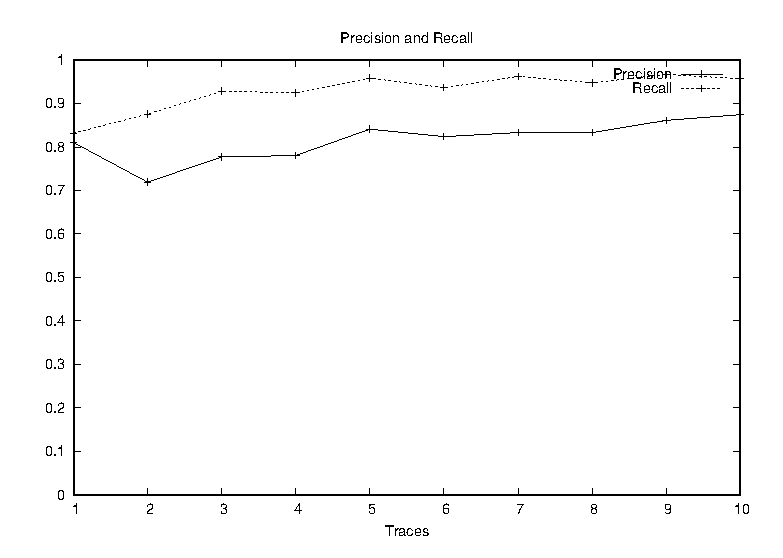
\includegraphics[width=0.65\linewidth]{figures/input_size_100_10_precision.eps}
	\caption{Precision and recall when learning from [1-10] plan traces with \FO action sequences and \PO state trajectories with 10\% observability.}
	\label{fig:np_quality}
\end{figure}

\begin{figure}[hbt!]
	\centering
	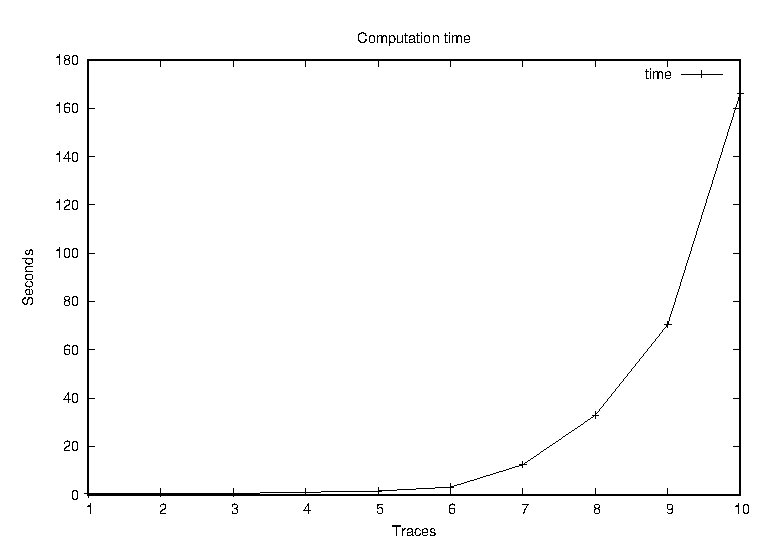
\includegraphics[width=0.65\linewidth]{figures/input_size_100_10_time.eps}
	\caption{Computation time when learning from [1-10] plan traces with \FO action sequences and \PO state trajectories with 10\% observability.}
	\label{fig:np_time}
\end{figure}

Figure~\ref{fig:pspace_quality} displays the average precision and recall of the 15 learned models in the scenario with unknown plan horizon. As expected, the quality of the learned models is lower than when the horizon of the plan is known. The higher complexity of this setting is also reflected in the appearance of some timeouts when solving the learning task. The first timeout is found in the \emph{grid} domain at $|\mathcal{T}| = 3$; the \emph{floortile} times out with $|\mathcal{T}| = 4$; and by the time $|\mathcal{T}|$ reaches 10 the number of domains where no solution is found is 6, adding the \emph{npuzzle, parking, rovers and zenotravel} domains. We can observe in Figure~\ref{fig:pspace_quality} the opposite behaviour to Figure~\ref{fig:np_quality}; that is, we find a drop of the quality as the input knowledge increases. The drop in the score is caused by the increasing number of timeouts, meaning that no solution is found in many tasks within the given time-bound, and consequently a value of $0$ for precision and recall is assigned to these experiments. Figure \ref{fig:pspace_time}, on the other hand, reflects that the computation time of the second case study is also higher than in the first case, which is explained by both the higher complexity and the large number of timeouts.


The conclusions we draw from these experiments is that, when the plan horizon is known, learning with few input samples yield action models that contain 95\% of the preconditions and effects of the GTM plus some extra ones as indicated by the values of precision and recall. With unknown plan horizons, on the other hand, the learned models are generally more different from the GTM; while timeouts are the main cause of the drop in the score, we must point out that pure syntax-based metrics are not adequate to evaluate such under-constrained tasks since the phenomenon of \emph{reformulation} occurs and this largely impacts the results (we will provide experimental evidence of this in section \ref{minimal}). These results emphasize a relevant feature our approach: the small size of the training set required by \FAMA in comparison with other approaches (see Table \ref{table:models_comparison2}). Unlike extensive-data approaches, our work explores an alternative research direction to learn action models from small amounts of plan traces. This is an important advantage, particularly in domains in which it is costly or impossible to obtain a significant number of training samples.


\begin{figure}[hbt!]
	\centering
	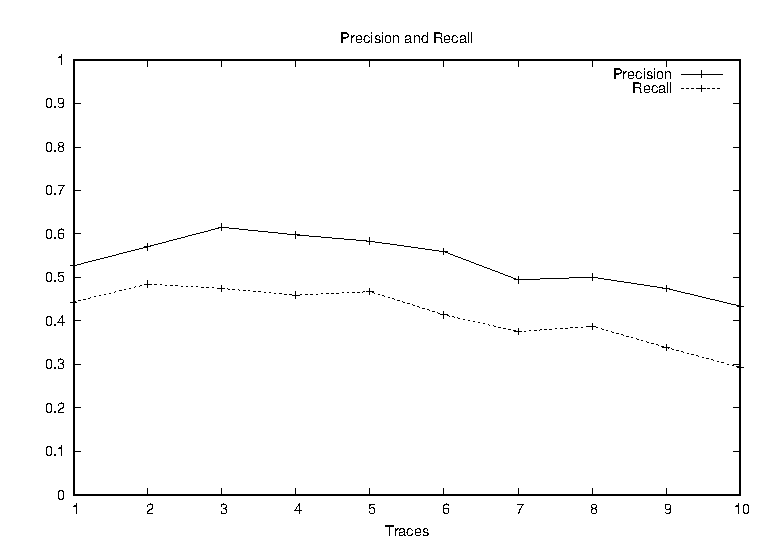
\includegraphics[width=0.65\linewidth]{figures/input_size_0_0_precision.eps}
	\caption{Precision and recall when learning from [1-10] plan traces with \NO action sequences and \NO state trajectories.}
	\label{fig:pspace_quality}
\end{figure}
\begin{figure}[hbt!]
	\centering
	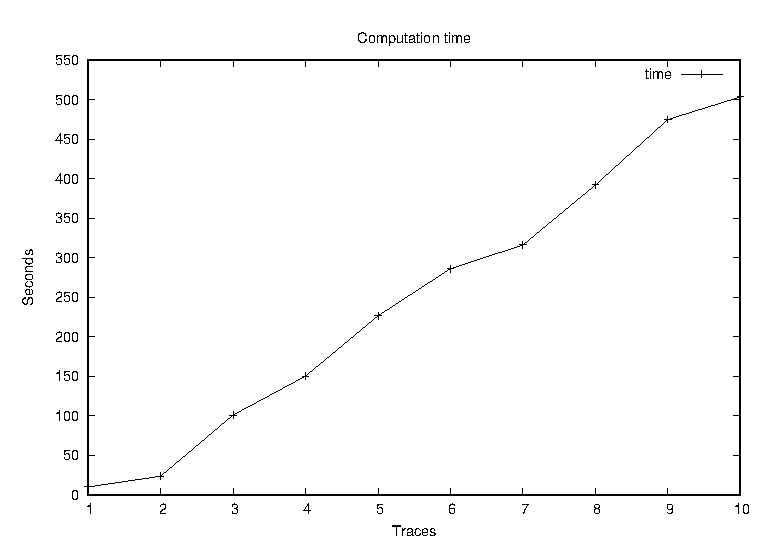
\includegraphics[width=0.65\linewidth]{figures/input_size_0_0_time.eps}
	\caption{Computation time when learning from [1-10] plan traces with \NO action sequences and \NO state trajectories.}
	\label{fig:pspace_time}
\end{figure}


\subsection{Comparison with \ARMS}
\label{compare_ARMS}

In this section we analyze the performance of \FAMA compared to \ARMS, one of the most well-known approaches to learning planning models. \ARMS, as well as most of the existing current learning systems, works under the assumption of plan traces with \FO action sequences and \NO state trajectories and therefore is not able to handle the scenarios where the plan horizon is unknown. We will thereby restrict the experimentation to the cases manageable by \ARMS.

In this experiment, we defined a \emph{degree of observability} $\sigma$ for the state trajectory, ranging from 0\% to 100\%, that measures the probability of observing a literal, and evaluated both \FAMA and \ARMS for increasing values of $\sigma$ using five traces as input knowledge. When $\sigma = 0$ we have a \NO state trajectory, when $\sigma=100$ we have a \FO state trajectory and all cases in-between correspond to the \PO scenario.

Figures \ref{fig:comparison_precision} and \ref{fig:comparison_recall} compare \FAMA and \ARMS in terms of precision and recall. The horizontal axes represent the degree of observability and vertical axes show the average precision (Figure \ref{fig:comparison_precision}) and recall (Figure \ref{fig:comparison_recall}) computed over the 15 tested domains. Remarkably, \FAMA dominates in terms of precision in all cases except for the \FO state trajectories. Particularly, the models learned by \FAMA are between 13\% to 34\% more precise than those learned by \ARMS. A similar trend is observed for recall (Figure \ref{fig:comparison_recall}), where the difference is even larger, meaning that our learned models are more complete.

The results highlight that \FAMA outperforms \ARMS when very few plan traces are available. This by no means is conclusive that \FAMA is overall better in NP-complete scenarios but only that it is able to learn better with very limited input knowledge (actually, Figure~\ref{fig:np_time} reflects the exponential behaviour of \FAMA with more than five traces).



\begin{figure}[hbt!]
	\centering
	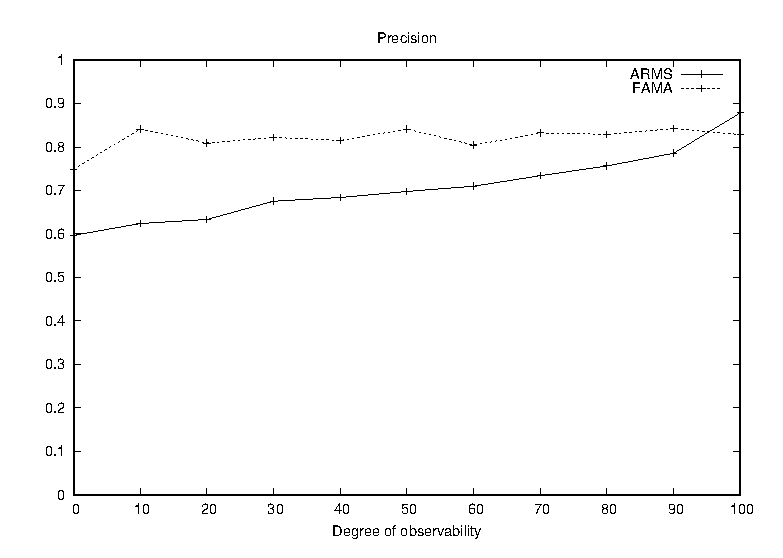
\includegraphics[width=.65\linewidth]{figures/comparison_precision.eps}
	\caption{Precision comparison between \FAMA and \ARMS for different \emph{degrees of observability}.}
	\label{fig:comparison_precision}
\end{figure}

\begin{figure}[hbt!]
	\centering
	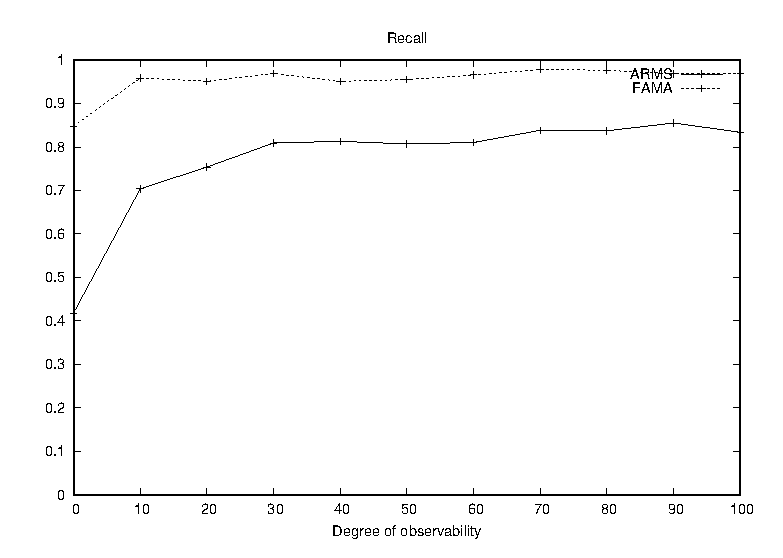
\includegraphics[width=.65\linewidth]{figures/comparison_recall.eps}
	\caption{Recall comparison between \FAMA and \ARMS for different \emph{degrees of observability}.}
	\label{fig:comparison_recall}
\end{figure}



\subsection{Learning with minimal input knowledge}
\label{minimal}


In this section, we will take a closer look at the action models learned from minimal input knowledge. To that end, we will limit the input to only two plan traces and analyze the results under different degrees of observability. We evaluate three case studies:

\begin{itemize}
	\item \textbf{\FO action sequence and \PO state trajectory}: We are, once again, assuming a degree of observability of 10\% for the state trajectory. Results of this case study are detailed in Table \ref{tab:results_minimum_100_10}.
	\item  \textbf{\PO action sequence and \PO state trajectory}: In this case study we are assuming a degree of observability of 30\% for both the action sequence and state trajectory. Results are shown in Table \ref{tab:results_minimum_30_30}.
	\item  \textbf{\NO action sequence and \NO state trajectory}: Both the action sequence and state trajectory are completely empty so only the initial and final states are observed; i.e., $\tau = \tup{s_0, s_m}, \forall \tau \in \mathcal{T}$. Results of this case study are reported in Table \ref{tab:results_minimum_0_0}.
\end{itemize}

All tables in this section (Tables \ref{tab:results_minimum_100_10}, \ref{tab:results_minimum_30_30} and \ref{tab:results_minimum_0_0}) follow the same structure. precision ({\bf P}) and recall ({\bf R}) scores are computed separately for the preconditions ({\bf Pre}), positive effects ({\bf Add}) and negative effects ({\bf Del}), and also globally ({\bf Global}). The last column reports the computation time (in seconds) needed to obtain the learned models. Missing values in the tables (reported as -) correspond to domains where no solution was found within a 1800s timeout.

Table \ref{tab:results_minimum_100_10} shows the results of the case study \FO/\PO. Recall scores are generally higher than the precision ones, and, in fact, the models learned for six out of the 15 domains were perfectly complete. Although precision is overall lower, it is interesting to notice that the learned sets of negative effects are mostly flawless. With regards to the computation time, we can observe times are below one second in most cases except for some of the more complex domains.

\begin{table}[hbt!]
		\begin{center}
                  \begin{footnotesize}			
			\begin{tabular}{l|l|l|l|l|l|l||l|l||l|}
				& \multicolumn{2}{|c|}{\bf Pre} & \multicolumn{2}{|c|}{\bf Add} & \multicolumn{2}{|c||}{\bf Del} & \multicolumn{2}{|c|}{\bf Global} & \\ \cline{2-9}			
				& \multicolumn{1}{|c|}{\bf P} & \multicolumn{1}{|c|}{\bf R} & \multicolumn{1}{|c|}{\bf P} & \multicolumn{1}{|c|}{\bf R} & \multicolumn{1}{|c|}{\bf P} & \multicolumn{1}{|c||}{\bf R} &  \multicolumn{1}{|c|}{\bf P} & \multicolumn{1}{|c|}{\bf R} & {\bf Time} \\
				\hline
				Blocks & 0.86 & 0.67 & 1.0 & 0.67 & 0.8 & 0.44 & 0.89 & 0.59& 0.24 \\ 
				Driverlog & 0.6 & 0.86 & 0.36 & 0.57 & 0.67 & 0.29 & 0.53 & 0.64& 0.58 \\
				Ferry & 0.7 & 1.0 & 0.36 & 1.0 & 1.0 & 1.0 & 0.6 & 1.0& 0.37 \\ 
				Floortile & 0.69 & 1.0 & 0.55 & 1.0 & 1.0 & 0.82 & 0.69 & 0.95& 1.38 \\
				Grid & 0.68 & 0.88 & 0.5 & 0.86 & 0.88 & 1.0 & 0.67 & 0.9& 0.65 \\ 
				Gripper & 1.0 & 1.0 & 1.0 & 1.0 & 1.0 & 1.0 & 1.0 & 1.0& 0.18 \\ 
				Hanoi & 0.67 & 1.0 & 1.0 & 1.0 & 1.0 & 1.0 & 0.8 & 1.0& 0.36 \\
				Miconic & 1.0 & 1.0 & 0.57 & 1.0 & 1.0 & 1.0 & 0.84 & 1.0& 0.3 \\ 
				Npuzzle & 0.75 & 1.0 & 1.0 & 1.0 & 1.0 & 1.0 & 0.88 & 1.0& 0.26 \\ 
				Parking & 0.78 & 1.0 & 0.69 & 1.0 & 1.0 & 1.0 & 0.8 & 1.0& 0.24 \\
				Rovers & 0.54 & 1.0 & 0.3 & 0.76 & 1.0 & 0.46 & 0.48 & 0.85 & 2.14 \\
				Satellite & 0.93 & 1.0 & 0.56 & 1.0 & 1.0 & 0.75 & 0.81 & 0.96& 0.4 \\ 
				Transport & 0.83 & 1.0 & 0.5 & 1.0 & 0.6 & 0.6 & 0.67 & 0.9& 0.19 \\
				Visitall & 1.0 & 1.0 & 0.25 & 0.5 & 1.0 & 1.0 & 0.57 & 0.8& 1.31 \\
				Zenotravel & 0.9 & 0.64 & 0.5 & 0.71 & 0.83 & 0.71 & 0.73 & 0.68& 0.25 \\ 
				\hline
				\bf & 0.8 & 0.94 & 0.61 & 0.87 & 0.92 & 0.8 & 0.73 & 0.88 & 0.59 \\
			\end{tabular}
                  \end{footnotesize}			
		\end{center}
	\caption{\small Precision and recall scores for learning tasks with \FO action sequences and \PO state trajectories with 10\% observability.}
	\label{tab:results_minimum_100_10}
\end{table}


Table \ref{tab:results_minimum_30_30} gathers the results of the case study \PO/\PO with 30\% observability.  We can see in the table that the scores of some domains are missing. This is the case of {\em floor-tile} and {\em grid}, which not only are fairly complex domains, but also categorized as \emph{puzzle-like} domains, a feature that is known for putting a strain in the planners. Interestingly enough, we note the high computation time of {\em hanoi} and {\em parking}, which also qualify as a \emph{puzzle-like} domains. Regarding quality, we find that the learned models retain a level of soundness similar to Table~\ref{tab:results_minimum_100_10} but the completeness is lower than in the previous case study. This is specially noticeable in the preconditions, where recall values drop from 0.88 to 0.64. This is because the input actions act as strong constraints playing a key role on the closeness of the learned model to the GTM. The more actions are missing in the input knowledge, the more likely the occurrence of reformulations.

\begin{table}[hbt!]
	\begin{center}
		\begin{footnotesize}
		\begin{tabular}{l|l|l|l|l|l|l||l|l||l|}
			& \multicolumn{2}{|c|}{\bf Pre} & \multicolumn{2}{|c|}{\bf Add} & \multicolumn{2}{|c||}{\bf Del} & \multicolumn{2}{|c|}{\bf Global} & \\ \cline{2-9}			
			& \multicolumn{1}{|c|}{\bf P} & \multicolumn{1}{|c|}{\bf R} & \multicolumn{1}{|c|}{\bf P} & \multicolumn{1}{|c|}{\bf R} & \multicolumn{1}{|c|}{\bf P} & \multicolumn{1}{|c||}{\bf R} &  \multicolumn{1}{|c|}{\bf P} & \multicolumn{1}{|c|}{\bf R} & {\bf Time} \\
			\hline
			Blocks & 0.89 & 0.89 & 0.8 & 0.89 & 0.83 & 0.56 & 0.84 & 0.78& 0.77 \\ 
			Driverlog & 0.57 & 0.29 & 0.31 & 0.57 & 0.4 & 0.29 & 0.4 & 0.36& 7.35 \\ 
			Ferry & 0.83 & 0.71 & 0.36 & 1.0 & 1.0 & 1.0 & 0.62 & 0.87& 3.38 \\ 
			Floortile & - & - & - & - & - & - & - & - & - \\ 
			Grid & - & - & - & - & - & - & - & - & - \\ 
			Gripper & 1.0 & 1.0 & 0.8 & 1.0 & 1.0 & 1.0 & 0.93 & 1.0& 0.17 \\ 
			Hanoi & 0.67 & 0.5 & 1.0 & 1.0 & 1.0 & 1.0 & 0.86 & 0.75& 132.69 \\ 
			Miconic & 1.0 & 0.33 & 1.0 & 1.0 & 1.0 & 0.67 & 1.0 & 0.56& 0.71 \\ 
			Npuzzle & 1.0 & 0.67 & 1.0 & 1.0 & 1.0 & 1.0 & 1.0 & 0.86& 13.48 \\ 
			Parking & 0.83 & 0.36 & 1.0 & 0.89 & 0.83 & 0.56 & 0.9 & 0.56& 160.64 \\
			Rovers & 0.43 & 0.73 & 0.24 & 0.47 & 0.56 & 0.38 & 0.39 & 0.61& 31.13 \\ 
			Satellite & 0.6 & 0.21 & 0.56 & 1.0 & 0.5 & 0.5 & 0.56 & 0.43& 11.55 \\ 
			Transport & 1.0 & 0.2 & 0.57 & 0.8 & 1.0 & 0.4 & 0.73 & 0.4& 23.39 \\ 
			Visitall & 0.67 & 1.0 & 0.5 & 0.5 & 1.0 & 1.0 & 0.67 & 0.8& 3.13 \\ 
			Zenotravel & 1.0 & 0.36 & 0.4 & 0.29 & 1.0 & 0.43 & 0.77 & 0.36& 226.27 \\
			\hline
			\bf & 0.81 & 0.56 & 0.66 & 0.8 & 0.86 & 0.68 & 0.74 & 0.64 & 47.28
			
		\end{tabular}
		\end{footnotesize}
	\end{center}
	\caption{\small Precision and recall when learning with \PO action sequences and \PO state trajectories, 30\% observability in both cases.}
	\label{tab:results_minimum_30_30}
\end{table}


We now analyze the case study with \NO action sequences and \NO state trajectories (Table~\ref{tab:results_minimum_0_0}). A first outstanding observation is that, contrary to what might be expected by looking at the previous table, we are able in this case to find solutions for all the domains. This happens because the search is less constrained and consequently there are far more possible solutions for this learning task. This broader space of solutions is also stressed in a diminished quality of the learned models. Thus, despite the learned models being consistent with the input data, they are further from the original GTM. In Table~\ref{tab:results_minimum_0_0} we can observe the global values of precision and recall drop to 0.57 and 0.48, respectively.

We argue, however, that syntax-based metrics are not appropriate for scenarios with minimal observability as they cannot cope with the reformulations that frequently occur in these circumstances. To illustrate this, Figure \ref{fig:macroaction} shows the PDDL encoding of the action model of the {\tt\small stack} operator learned from plan traces with \NO action sequences and \NO state trajectories. This learned action model removes a block from on top of another block and puts it down on the table in a single step. There are two main differences with respect to the model of the {\tt\small stack} operator of the GTM: (1) the learned action is actually \emph{unstacking} a block instead of stacking it and (2) the block on the top ends on the table, not held by the robot arm. We refer to the first difference as \emph{role swapping} and it happens when there are missing actions in the input plan trace. If no actions are present in the input traces, the names of actions become meaningless, in which case the effectively anonymous actions can interchange their behaviour with any other comparable action model. The second difference indeed reveals that the learned action model is working as an {\tt\small unstack+put-down} \emph{macro-action}. This happens when there are missing states in the input traces since a \emph{macro-action} can be seen as the application of more than one action in a single step, thus skipping some intermediate states.

Reformulated action models, like the one in Figure \ref{fig:macroaction}, are indeed sound models that can be used to solve planning tasks. For instance, any \emph{blocks-world} problem can be solved unstacking all the blocks to the table ({\tt\small unstack+put-down}) and then stacking them to meet the goal conditions ({\tt\small pick-up+stack}). Hence, the \NO/\NO case study features all the conditions for reformulation to happen, and this is the reason why scenarios such as this one are better evaluated using {\em semantic-based metrics}.


\begin{table}[hbt!]
  \begin{center}
    \begin{footnotesize}
		\begin{tabular}{l|l|l|l|l|l|l||l|l||l|}
			& \multicolumn{2}{|c|}{\bf Pre} & \multicolumn{2}{|c|}{\bf Add} & \multicolumn{2}{|c||}{\bf Del} & \multicolumn{2}{|c|}{\bf Global} & \\ \cline{2-9}			
			& \multicolumn{1}{|c|}{\bf P} & \multicolumn{1}{|c|}{\bf R} & \multicolumn{1}{|c|}{\bf P} & \multicolumn{1}{|c|}{\bf R} & \multicolumn{1}{|c|}{\bf P} & \multicolumn{1}{|c||}{\bf R} &  \multicolumn{1}{|c|}{\bf P} & \multicolumn{1}{|c|}{\bf R} & {\bf Time} \\
			\hline
			Blocks & 0.6 & 0.67 & 0.33 & 0.22 & 0.67 & 0.44 & 0.55 & 0.44& 0.26 \\ 
			Driverlog & 0.5 & 0.29 & 0.33 & 0.57 & 0.0 & 0.0 & 0.38 & 0.29& 0.88 \\
			Ferry & 0.5 & 0.43 & 0.5 & 0.25 & 0.67 & 0.5 & 0.55 & 0.4& 0.45 \\ 
			Floortile & 0.48 & 0.45 & 0.27 & 0.36 & 0.46 & 0.55 & 0.41 & 0.45& 58.38 \\
			Grid & 0.25 & 0.24 & 0.33 & 0.43 & 0.14 & 0.14 & 0.25 & 0.26& 234.63 \\ 
			Gripper & 1.0 & 0.67 & 1.0 & 1.0 & 1.0 & 1.0 & 1.0 & 0.86& 0.16 \\ 
			Hanoi & 0.6 & 0.75 & 1.0 & 1.0 & 1.0 & 1.0 & 0.78 & 0.88& 6.32 \\ 
			Miconic & 0.63 & 0.56 & 0.6 & 0.75 & 0.25 & 0.33 & 0.53 & 0.56& 0.25 \\ 
			Npuzzle & 1.0 & 1.0 & 1.0 & 1.0 & 1.0 & 1.0 & 1.0 & 1.0& 1.52 \\ 
			Parking & 0.57 & 0.29 & 0.2 & 0.11 & 0.8 & 0.44 & 0.53 & 0.28& 17.43 \\
			Rovers & 0.38 & 0.64 & 0.07 & 0.24 & 0.13 & 0.54 & 0.22 & 0.53& 1.74 \\
			Satellite & 0.86 & 0.43 & 0.43 & 0.6 & 0.75 & 0.75 & 0.67 & 0.52& 3.15 \\
			Transport & 0.29 & 0.2 & 0.38 & 0.6 & 0.67 & 0.4 & 0.39 & 0.35& 1.06 \\
			Visitall & 0.0 & 0.0 & 1.0 & 0.5 & 0.0 & 0.0 & 1.0 & 0.2& 1.21 \\ 
			Zenotravel & 0.4 & 0.29 & 0.25 & 0.29 & 0.2 & 0.14 & 0.3 & 0.25& 17.48 \\ 			
			\hline
			\bf & 0.54 & 0.46 & 0.51 & 0.53 & 0.52 & 0.48 & 0.57 & 0.48 & 22.99
		\end{tabular}
            \end{footnotesize}
	\end{center}
	\caption{\small Precision and recall scores for learning tasks with \NO action sequences and \NO state trajectories.}
	\label{tab:results_minimum_0_0}
\end{table}


\begin{figure}[hbt!]
	\begin{footnotesize}
		\begin{verbatim}
(:action stack
 :parameters (?o1 - object ?o2 - object)
 :precondition (and (on ?o1 ?o2)(handempty ))
 :effect (and (not (on ?o1 ?o2))(clear ?o1)(clear ?o2)(ontable ?o1)))
		\end{verbatim}
	\end{footnotesize}
	\caption{PDDL encoding of the learned action model of the {\em stack} operator from the four-operator {\em blocksworld} domain.}
	\label{fig:macroaction}
\end{figure}



\subsection{Syntactic versus semantic evaluation}
\label{semantic}

Our last experiment is devoted to compare the scores provided by the syntactic and semantic versions of precision and recall. For that purpose, we will evaluate the models learned in Section \ref{minimal} both syntactically, using the GTM, and semantically, computing the set of action models closest to the learned models that is consistent with a testing set of five traces (see Definition \ref{compliant}). We must note that since we are using {\sc Madagascar}, a satisficing planner, the solution to the model evaluation may not be the closest consistent domain model, so the scores of sem-Precision and sem-Recall are approximate values. Our goal with this experiment is to gauge the suitability of the semantic metrics proposed in section \ref{sec:evaluation} with respect to their well-known counterparts. With that in mind, we define two case studies:

\begin{itemize}
	\item \textbf{\FO action sequence and \PO state trajectory}: In this case study the full sequence of actions is known and no states are missing, which makes it practically impossible for reformulated models to appear. In fact, in all our experimentation with \FAMA and other approaches we never observed reformulations when the full sequence of actions is known.
	\item  \textbf{\NO action sequence and \NO state trajectory}: This is a case study that favors reformulations in the learned models, as previously discussed.
\end{itemize}

\begin{table}[hbt!]
     \begin{footnotesize}
	 \begin{center}		
		\begin{tabular}{l|c|c|c|c|}		
			& {\bf Precision} & {\bf Recall} & {\bf sem-Precision} & {\bf sem-Recall} \\
			\hline
			Blocks & 0.89 & 0.59 & 0.89 & 0.64 \\
			Driverlog & 0.53 & 0.64 & 0.71 & 0.83 \\
			Ferry & 0.6 & 1.0 & 0.96 & 1.0 \\
			Floortile & 0.69 & 0.95 & 0.97 & 0.95 \\
			Grid & 0.67 & 0.9 & 0.95 & 0.98 \\
			Gripper & 1.0 & 1.0 & 1.0 & 1.0 \\
			Hanoi & 0.8 & 1.0 & 0.9 & 1.0 \\
			Miconic & 0.84 & 1.0 & 1.0 & 1.0 \\
			Npuzzle & 0.88 & 1.0 & 1.0 & 1.0 \\
			Parking & 0.8 & 1.0 & 0.98 & 1.0 \\
			Rovers & 0.48 & 0.85 & 0.94 & 0.99 \\
			Satellite & 0.81 & 0.96 & 0.93 & 1.0 \\
			Transport & 0.67 & 0.9 & 1.0 & 1.0 \\
			Visitall & 0.57 & 0.8 & 1.0 & 1.0 \\
			Zenotravel & 0.73 & 0.68 & 0.85 & 0.88 \\
			\hline
			& 0.73 & 0.88 & 0.94 & 0.95
		\end{tabular}
	 \end{center}
     \end{footnotesize}
     \caption{\small Syntactic and semantic scores when learning with \FO action sequences and \PO state trajectories with 10\% observability.}
     \label{tab:metric_comparison_100_10}
\end{table}


Table \ref{tab:metric_comparison_100_10} shows the results of the case study \FO/\PO. Looking at the high scores of the syntactic metrics, specially the value of recall, we can conclude that the learned models are, in fact, fairly similar to the GTM. This supports our conclusion that no reformulation occurs in this case study, which also means that the space of possible solutions is restricted to models close to the GTM. The values of sem-Precision and sem-Recall are also very high across the table, which is exactly the desired behavior for these metrics given that solutions are very close to the GTM. In comparison, recall and sem-Recall show similar scores, while sem-Precision is significantly higher than precision, thus showing that the sem-Precision is more lenient towards extra preconditions or effects. This is in line with the results of the previous experiments, where the common appearance of redundant or implicit preconditions in the learned models is penalized by the precision metric. We can interpret this phenomenon as a manifestation of the qualification problem~\cite{GinsbergS88}. For instance, the model learned for the {\tt\small move} action of the {\em hanoi} domain specifies that both the origin and destination disks must be bigger than the one moving, but the GTM contains only one of these preconditions. This learned model is semantically correct but syntactically different from the GTM and hence penalized by the precision metric.

Table~\ref{tab:metric_comparison_0_0} details the results of the case study \NO/\NO. One first observation is the impossibility of applying a semantic evaluation in some of the most complex domains with five traces. Contrary to the previous case study, the difference between the syntactic and semantic metrics is larger in this scenario with unknown plan horizon. Comparing the scores of both versions, we find that learned models that achieved mediocre scores when using the GTM as reference (syntactic metrics), are in fact reasonably sound and complete, reaching overall scores of 0.92 and 0.89 in sem-Precision and sem-Recall. This is an indication that the models learned by our approach, despite syntactically different from the GTM, require very few editions to explain the testing set of traces.

\begin{table}[hbt!]
    \begin{footnotesize}
	\begin{center}		
		\begin{tabular}{l|c|c|c|c|}		
			& {\bf Precision} & {\bf Recall} & {\bf sem-Precision} & {\bf sem-Recall} \\
			\hline
			Blocks & 0.55 & 0.44 & 0.77 & 0.77 \\
			Driverlog & 0.38 & 0.29 & 0.86 & 0.86 \\
			Ferry & 0.55 & 0.4 & 0.82 & 0.53 \\
			Floortile & 0.41 & 0.45 & - & - \\
			Grid & 0.25 & 0.26 & - & - \\
			Gripper & 1.0 & 0.86 & 1.0 & 1.0 \\
			Hanoi & 0.78 & 0.88 & 0.89 & 1.0 \\
			Miconic & 0.53 & 0.56 & 1.0 & 0.89 \\
			Npuzzle & 1.0 & 1.0 & 1.0 & 1.0 \\
			Parking & 0.53 & 0.28 & - & - \\
			Rovers & 0.22 & 0.53 & - & - \\
			Satellite & 0.67 & 0.52 & - & - \\
			Transport & 0.39 & 0.35 & 0.94 & 1.0 \\
			Visitall & 1.0 & 0.2 & 1.0 & 1.0 \\
			Zenotravel & 0.3 & 0.25 & - & - \\
			\hline
			& 0.57 & 0.48 & 0.92 & 0.89
		\end{tabular}
	\end{center}
    \end{footnotesize}
	\caption{\small Syntactic and semantic metric scores for learning tasks with \NO action sequences and \NO state trajectories.}
	\label{tab:metric_comparison_0_0}
\end{table}

Looking at the results of both case studies we can draw two conclusions with regards to the semantic metrics proposed in this paper. The first one is that, when no reformulation occurs, these metrics behave similarly to their syntactic counterparts, which means they are a good substitute when the GTM is not available. The second conclusion is that sem-Precision and sem-Recall are better suited to evaluate reformulated models than the original syntactic metrics since they contemplate valid solutions outside the GTM that successfully explain the given input data.
